\documentclass[journal]{IEEEtran}

% Additional packages
\usepackage{graphicx}
\usepackage{amsmath}
\usepackage{hyperref}
\usepackage{qrcode}
\usepackage{float}

\begin{document}

\title{Determination of Resistance by Wheatstone Bridge Method}
\author{IBRAHIM H.I. ABUSHAWISH\\
Istanbul University Physics Department\\
Instructor: \hspace{10px} \\
Experiment Date: 07.10.2024 , Report Submission Date: 14.10.2024\\
Course \& Section Number: PHYS2305}

\maketitle

\begin{abstract}
    This experiment investigates the determination of an unknown resistance using the Wheatstone Bridge method. The relationship between resistance, resistivity, length, and cross-sectional area is explored through experimental procedures and theoretical analysis. The results demonstrate the accuracy and reliability of the Wheatstone Bridge in measuring unknown resistances.
\end{abstract}

\section{Introduction}
The Wheatstone Bridge is a fundamental circuit used to measure unknown resistances. This experiment aims to demonstrate the principles of resistance measurement and the calculation of resistivity based on the geometry of the conductor. The Wheatstone Bridge configuration allows for precise determination of an unknown resistance by balancing two legs of a bridge circuit.

\section{Theory}
The resistance $$ R $$ of a conductor is given by the formula:
$$
R = \rho \frac{L}{A}
$$
where $$ \rho $$ is the resistivity, $$ L $$ is the length, and $$ A $$ is the cross-sectional area. The Wheatstone Bridge configuration allows for the calculation of an unknown resistance $$ R_1 $$ using known resistances $$ R_2 $$, $$ R' $$, and $$ R'' $$ as follows:
$$
\frac{R_1}{R_2} = \frac{R'}{R''}
$$

\section{Experimental Setup}
The experimental setup consists of a Wheatstone Bridge circuit, a galvanometer, a voltage source, and a variable resistor. The circuit is arranged as shown in Figure \ref{fig:wheatstone_bridge}.

\begin{figure}[H]
    \centering
    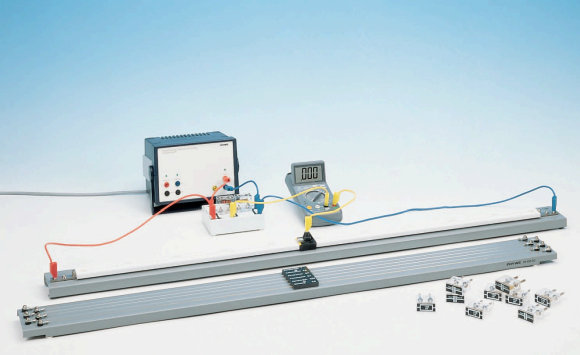
\includegraphics[width=0.5\textwidth]{IMAGES/wheatstone_bridge.png} % Replace with your figure
    \caption{Wheatstone Bridge Circuit \cite{lab_report}}
    \label{fig:wheatstone_bridge}
\end{figure}

\section{Procedure}
\begin{enumerate}
    \item Set up the Wheatstone Bridge circuit as illustrated.
    \item Adjust the variable resistor until the galvanometer reads zero current, indicating equilibrium.
    \item Record the lengths $$ L' $$ and $$ L'' $$ of the resistors used.
    \item Calculate the unknown resistance $$ R_1 $$ using the measured lengths and known resistances.
\end{enumerate}

\section{Results}
Present your results in a table format, similar to Table \ref{tab:results}.

\begin{table}[H]
    \centering
    \begin{tabular}{|c|c|c|c|}
        \hline
        $ R_1  (k\Omega)$ & $ R_2  (k\Omega)$ & $ L'  (cm)$ & $ L''  (cm)$ \\
        \hline
        82 & 100 & 30 & 40 \\
        4.7 & 10 & 15 & 20 \\
        330 & 150 & 25 & 35 \\
        \hline
    \end{tabular}
    \caption{Measured Values}
    \label{tab:results}
\end{table}

\section{Discussion}
Discuss the significance of the results, any discrepancies observed, and how they relate to the theoretical predictions. The accuracy of the Wheatstone Bridge method in determining unknown resistances is evaluated, and potential sources of error are identified.

\section{Conclusion}
Summarize the findings of the experiment and their implications for understanding resistance measurement. The Wheatstone Bridge method is confirmed to be a reliable and accurate technique for measuring unknown resistances.

\section{References}
\begin{thebibliography}{9}
    \bibitem{ref1} Author, A. (Year). \textit{Title of the source}. Publisher.
    \bibitem{lab_report} Istanbul University, Physics Laboratory II Experiment Book: Electricity and Magnetism, Department of Physics, 2024.
\end{thebibliography}

\end{document}